\chapter*{Pr�paration des routes}

\section{Objet}
 L'objet de cette section est de d�crire les diff�rentes �tapes de pr�paration d'une route : choix des cartes, 
  d�finition des waypoints, trac� de la route, rep�rage des dangers, calculs des distances, sauvegarde et simulation du trajet.
\hbox{}\vspace{0.2cm}


\hbox{}\vspace{0.2cm}
\section{Choix des cartes}

%%%%%%%%%%%%%%%%%%%%%%%%%%%%%%%%%%%%%%%%%%%%%%%%%%%%%%%%%%%%%%%%%%%%%%%
	\begin{center}
		\framebox[1\width]{
			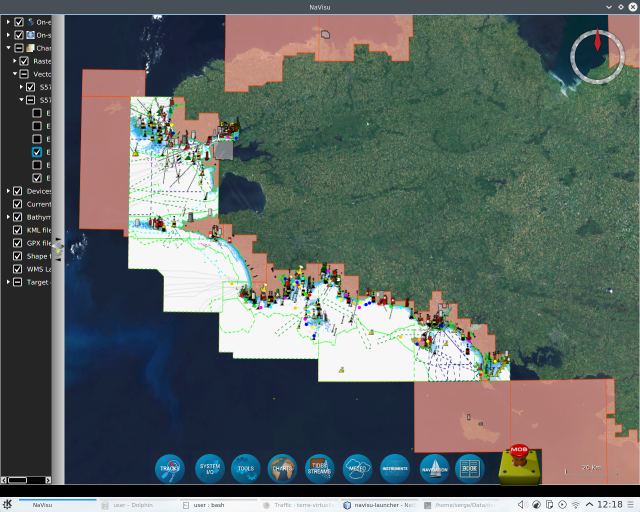
\includegraphics[width=12cm]{images/routes/route_0.png}
		}
		\begin{figure}[ht]
			\caption{\label{0}\textit{Choix des cartes � partir du catalogue ou directement}}
		\end{figure}
	\end{center}
%%%%%%%%%%%%%%%%%%%%%%%%%%%%%%%%%%%%%%%%%%%%%%%%%%%%%%%%%%%%%%%%%%%%%%%
\section{S�lection du menu RouteEditor}
%%%%%%%%%%%%%%%%%%%%%%%%%%%%%%%%%%%%%%%%%%%%%%%%%%%%%%%%%%%%%%%%%%%%%%%
	\begin{center}
		\framebox[1\width]{
			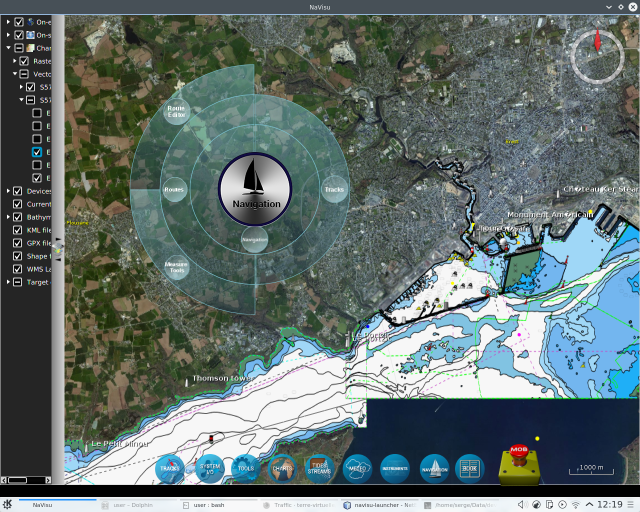
\includegraphics[width=12cm]{images/routes/route_1.png}
		}
		\begin{figure}[ht]
			\caption{\label{0}\textit{Menu Navigation : l'�diteur de routes}}
		\end{figure}
	\end{center}
%%%%%%%%%%%%%%%%%%%%%%%%%%%%%%%%%%%%%%%%%%%%%%%%%%%%%%%%%%%%%%%%%%%%%%%	%%%%%%%%%%%%%%%%%%%%%%%%%%%%%%%%%%%%%%%%%%%%%%%%%%%%%%%%%%%%%%%%%%%%%%%
		\begin{center}
			\framebox[1\width]{
				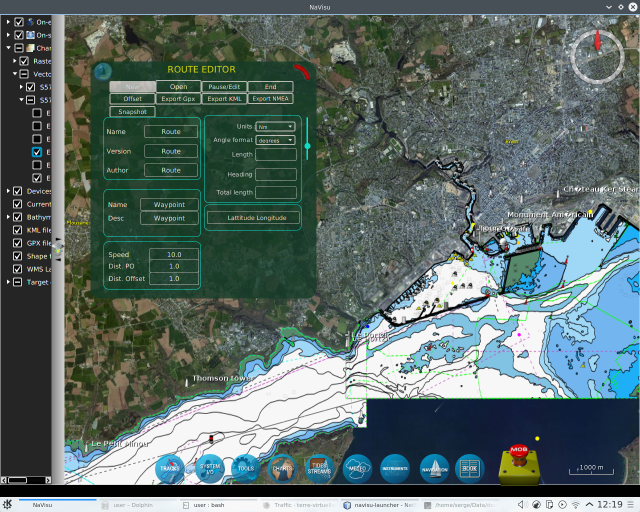
\includegraphics[width=12cm]{images/routes/route_2.png}
			}
			\begin{figure}[ht]
				\caption{\label{0}\textit{Menu RouteEditor : les param�tres de la route}}
			\end{figure}
		\end{center}
%%%%%%%%%%%%%%%%%%%%%%%%%%%%%%%%%%%%%%%%%%%%%%%%%%%%%%%%%%%%%%%%%%%%%%%
%%%%%%%%%%%%%%%%%%%%%%%%%%%%%%%%%%%%%%%%%%%%%%%%%%%%%%%%%%%%%%%%%%%%%%%
			\begin{center}
				\framebox[1\width]{
					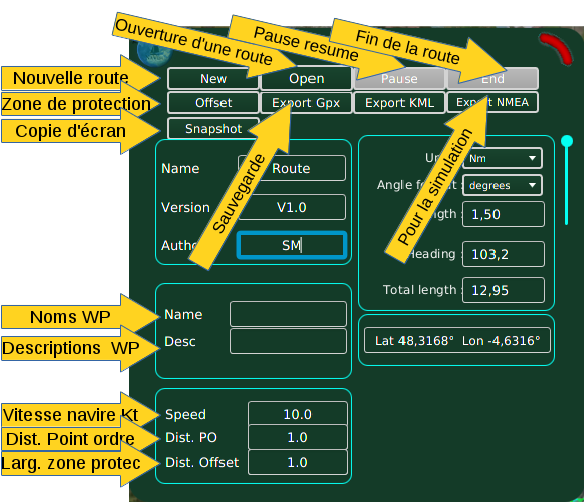
\includegraphics[width=12cm]{images/routes/routeeditor_1.png}
				}
				\begin{figure}[ht]
					\caption{\label{0}\textit{Menu RouteEditor : les items}}
				\end{figure}
			\end{center}
%%%%%%%%%%%%%%%%%%%%%%%%%%%%%%%%%%%%%%%%%%%%%%%%%%%%%%%%%%%%%%%%%%%%%%%
\subsection{Le menu RouteEditor}

\begin{itemize}
	\item Les commandes
		\begin{itemize}
		\item Le bouton {\tt New} : d�but de la d�finition d'une route.
		\item Le bouton {\tt Open} : ouverture d'une route sauvegard�e au format Gpx.
		\item Le bouton {\tt Pause } : permet de se d�placer interactivement dans les cartes sans marquer de waypoint, {\tt Resume} permet de revenir au mode �dition.
		\item Le bouton {\tt End } : termine une route, il doit �tre imp�rativement presser en fin de route.
		\item Le bouton {\tt Offset} : permet de d�finir une zone de s�curit� autour de la route.
		\item Le bouton {\tt Export Gpx} : sauvegarde de la route, et si elle d�finie de la zone de s�curit�, sous format Gpx.
		\item Le bouton {\tt Export Kml} : sauvegarde de la route au format KML.
		\item Le bouton {\tt Export NMEA} : sauvegarde de la route sous forme de phrases NMEA, pour une simulation de d�placement.
		\item Le bouton {\tt Snapshot} : copie d'�cran.
		\end{itemize}
	\item Les donn�es utilisateur
		\begin{itemize}
			\item Les fichiers
			\begin{itemize}		
			 	\item Le champs {\tt Name }: d�finit les noms des fichiers de sauvegarde aux formats GPX, KML, NMEA. Ces fichiers sont dans les r�pertoires {\tt data/gpx, data/kml, data/nmea} respectivement.
			    \item Le champs {\tt Version } : num�ro de version dans le fichier GPX.
				\item Le champs {\tt Author }: nom de l'auteur dans le fichier Gpx.
			\end{itemize}
			\item Les Waypoints
			\begin{itemize}
				\item Le champs {\tt Name }: Par d�faut les waypoints se nomme WP0, WP1, \ldots Il est possible de leur donner un nom particulier.
				\item Le champs {\tt Desc. } Texte de description du waypoint.
		     \end{itemize}
		     \item La route
		     \begin{itemize}
		     	\item Le champs {\tt Speed }: vitesse moyenne du navire.
		     	\item Le champs {\tt Dist. point d'ordre } : distance permettant de d�finir un waypoint d'alerte pour changement de cap.
		     	\item Le champs {\tt Dist. offset }: d�finit la largeur de la bande de s�curit� entourant la route.
		     \end{itemize}
		     \end{itemize}
	 \item L'affichage
	  \begin{itemize}
	  	\item -
	  \end{itemize}
\end{itemize}
%%%%%%%%%%%%%%%%%%%%%%%%%%%%%%%%%%%%%%%%%%%%%%%%%%%%%%%%%%%%%%%%%%%%%%%
\section{Trac� de la route}
%%%%%%%%%%%%%%%%%%%%%%%%%%%%%%%%%%%%%%%%%%%%%%%%%%%%%%%%%%%%%%%%%%%%%%%
\begin{center}
	\framebox[1\width]{
		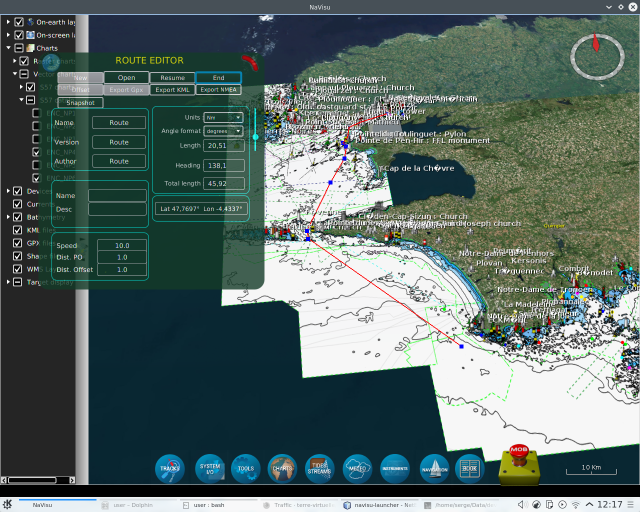
\includegraphics[width=16cm]{images/routes/route_3.png}
	}
	\begin{figure}[ht]
		\caption{\label{0}\textit{Trac� de la route}}
	\end{figure}
\end{center}
%%%%%%%%%%%%%%%%%%%%%%%%%%%%%%%%%%%%%%%%%%%%%%%%%%%%%%%%%%%%%%%%%%%%%%%

